\documentclass[10pt,a4paper]{report}
\usepackage[latin1]{inputenc}
\usepackage{amsmath}
\usepackage{amsfonts}
\usepackage{amssymb}
\usepackage{graphicx}
\usepackage{hyperref}
\usepackage{multicol}
\usepackage[margin=0.5in]{geometry}
\usepackage{tikz}
\usepackage[document]{ragged2e}
\usepackage{romannum}
\usetikzlibrary{arrows,shapes.gates.logic.US,shapes.gates.logic.IEC,calc}
\usepackage{titlesec}
\titlespacing{\subsection}{1pt}{\parskip}{3pt}
\titlespacing{\subsubsection}{0pt}{\parskip}{-\parskip}
\titlespacing{\paragraph}{0pt}{\parskip}{\parskip}
\newcommand{\myvec}[1]{\ensuremath{\begin{pmatrix}#1\end{pmatrix}}}



\begin{document}



\begin{multicols}{2}
\raggedright {
\includegraphics[scale=0.06]{IITH logo.jpg}} \vspace{3mm}\\ \raggedleft Name:SHAIK KHAJA MASTAN AHMED\vspace{2mm}\\ \raggedleft Roll No.: FWC22052\vspace{2mm}\\ \raggedleft 19pa1a04e9@vishnu.edu.in \vspace{2mm}\\ \raggedleft Sep 2022 \vspace{5mm}\\

\end{multicols}
\centering \Large \textbf{MATRIX: LINE ASSIGNMENT} \normalsize \vspace{10mm}

\begin{multicols}{2}

\section{Problem:}  
Construct a triangle XYZ in which $\angle{Y}=30^0$, $\angle{Z}=90^0$ and  XY+YZ+ZX=11cm.\vspace{2mm}

\section{Solution: }
\raggedright \textbf{Input Parameters:}\\
\vspace{1mm}
\begin{center}
\begin{tabular}{|c|c|c|}
	\hline
	\textbf{Symbol}&\textbf{Value}&\textbf{Description}\\
	\hline
	XY+YZ+ZX & 11cm & D\\
	\hline 
	$\angle{Z}$ & $90^0$ & Angle at Z \\
	\hline
	$\angle{Y}$ & $30^0$ & Angle at Y \\
	\hline
	
\end{tabular}
\end{center}
\vspace{3mm}



\raggedright Termux Command:\\
               \centering bash rncom.sh (Using Shell)\\
               \vspace{3mm} 

\raggedright \textbf{To Prove:}\\ \vspace{3mm} 
   Given, $\angle{Y}=30^0$, $\angle{Z}=90^0$ and  XY+YZ+ZX = Dcm.\\ \vspace{1mm}
   if $\angle{Y}=30^0$ and $\angle{Z}=90^0$ then $\angle{X}=60^0$\\
   Let us consider the coordinates of Y are X0,Y0 be $\begin{pmatrix}
  0\\
  0 \\
 \end{pmatrix}$% 
 \vspace{1mm} \\ Let 'z' be the distance between X and Y.
 \vspace{1mm} \\ Let the coordinates of X be X1,Y1 respectively.
  \\ \centering i.e., X = z$\begin{pmatrix}
  cos \theta\\
  sin \theta \\
 \end{pmatrix}$% 
 \vspace{2mm}
  \\ \raggedright And the coordinates of Z be X2,Y2 respectively.
  \\ \centering i.e., Z = z$\begin{pmatrix}
  cos \theta\\
  0 \\
 \end{pmatrix}$%
 \vspace{2mm}  \\So, by finding the values of coordinates of the all sides we can form a required triangle. \\
\vspace{2mm}
\raggedright \textbf{Finding the Coordinates: } \\
        \raggedright Given that XY+YZ+ZX=D. \frenchspacing \\
        \raggedright i.e., $||X-Y||$ + $||Y-Z||$ + $||Z-X||$ =D. \\ \vspace{1mm}
 $\implies$ z + zcos$\theta$+ zsin$\theta$ =D\\  
	\begin{center}	
	$\implies$ z = $\frac{D}{1+cos\theta+sin\theta}$
	\end{center}
\centering By solving we get 'z' , [$\because$ $\theta=30^0$ and D=11cm].\\ \vspace{2mm}
 $\therefore$ \text{z = 4.64} .\\ 
\raggedright Calculating the required vertices: \\ \vspace{2mm}
\centering X = z$\begin{pmatrix} 
  cos \theta\\
  sin \theta\\
 \end{pmatrix}$ =4.64 $\begin{pmatrix} 
  cos30^0\\
  sin30^0\\
 \end{pmatrix}$ = $\begin{pmatrix}
                 4.02\\
                 2.32\\
              \end{pmatrix}$ \\ \vspace{2mm}
\centering Z = z$\begin{pmatrix} 
  cos \theta\\
  0\\
 \end{pmatrix}$ = 4.64 $\begin{pmatrix} 
  cos30^0\\
  0\\
 \end{pmatrix}$ = $\begin{pmatrix}
                  4.02\\
                  0\\
              \end{pmatrix}$\\ \vspace{2mm}
\raggedright $\therefore$ The vertices of the required $\Delta$XYZ are:\\ \vspace{2mm}
\centering X= $\begin{pmatrix}
                 4.02\\
                 2.32\\
              \end{pmatrix}$%
              , Y= $\begin{pmatrix}
                 0\\
                 0\\
              \end{pmatrix}$% 
               , Z= $\begin{pmatrix}
                  4.02\\
                  0\\
              \end{pmatrix}$% 
 \vspace{3mm}             
\\
\textbf{The below python code realizes construction:}\\
https://github.com/19pa1a04e9/FWC-IITH/tree/main/Assignment-1/MATRICES/Line/line.py
  
 \section{Plot:}
 	\begin{center}
  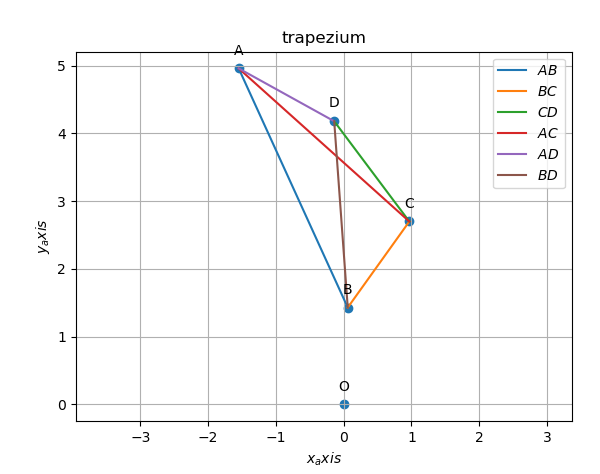
\includegraphics[scale=0.55]{line.png}
  	\end{center}
  


  



\vspace{3cm}

\end{multicols}

\end{document}
